\documentclass[shownotes]{beamer}

%
% Choose how your presentation looks.
%
% For more themes, color themes and font themes, see:
% http://deic.uab.es/~iblanes/beamer_gallery/index_by_theme.html
%
\mode<presentation>
{
  \usetheme{Madrid}      % or try Darmstadt, Madrid, Warsaw, ...
  \usecolortheme{default} % or try albatross, beaver, crane, ...
  \usefonttheme{default}  % or try serif, structurebold, ...
  \setbeamertemplate{navigation symbols}{}
  \setbeamertemplate{caption}[numbered]
}
\usepackage[utf8]{inputenc} %Para acentos en UTF8 (Prueba: á é í ó ú Á É Í Ó Ú ñ Ñ)
\usepackage[spanish]{babel}
\usepackage{cite}
\usepackage[utf8]{inputenc}
\usepackage{url}
\usepackage{graphicx}
\usepackage{caption}
\usepackage{float} % para que los gr\'aficos se queden en su lugar con [H]
\usepackage{subcaption}
\usepackage{wrapfig}
\usepackage{color}
\usepackage{amsmath} %para escribir funci\'on partida
\usepackage{hyperref} % para inlcuir links dentro del texto
\usepackage{tabu} 
\usepackage{amsmath}
\usepackage{comment}
\usepackage{amsfonts} % mathbb{N} -> conjunto de los n\'umeros naturales  
\usepackage{enumerate}
\usepackage{listings}

\captionsetup[figure]{labelformat=empty}

\hypersetup{
    colorlinks=true,       % false: boxed links; true: colored links
    linkcolor=white,          % color of internal links (change box color with linkbordercolor)
    citecolor=green,        % color of links to bibliography
    filecolor=magenta,      % color of file links
    urlcolor=cyan           % color of external links
}

% http://latexcolor.com/
\definecolor{lightseagreen}{rgb}{0.13, 0.7, 0.67}
\definecolor{tangelo}{rgb}{0.98, 0.3, 0.0}
\definecolor{git}{rgb}{0.94, 0.309, 0.2}

\setbeamercolor{structure}{fg=lightseagreen}

\newenvironment{ejercicio}[1]{
% \setbeamercolor{block title}{bg=tangelo, fg=white}
\begin{exampleblock}{#1}
}{
\end{exampleblock}
}

\newenvironment{resumen}[1]{
\setbeamercolor{block title}{bg=git, fg=white}
\begin{block}{#1}
}{
\end{block}
}

\newenvironment{comando}{
\setbeamercolor{block body}{bg=git, fg=white}
\begin{block}{}
\begin{center}
\LARGE
\begin{texttt}
}{
\end{texttt}
\end{center}
\end{block}
}



\title{Q learning}

\author{Socio Fisica}
\institute[DC-UBA]{FCEyN - UBA}
\date{\today}

\usepackage{Sweave}
\begin{document}
\input{qlearning-concordance}


\begin{frame}

\titlepage
  
\end{frame}

\begin{frame}{}


\begin{figure}[H]
    \centering
    \begin{subfigure}[b]{0.45\textwidth}
      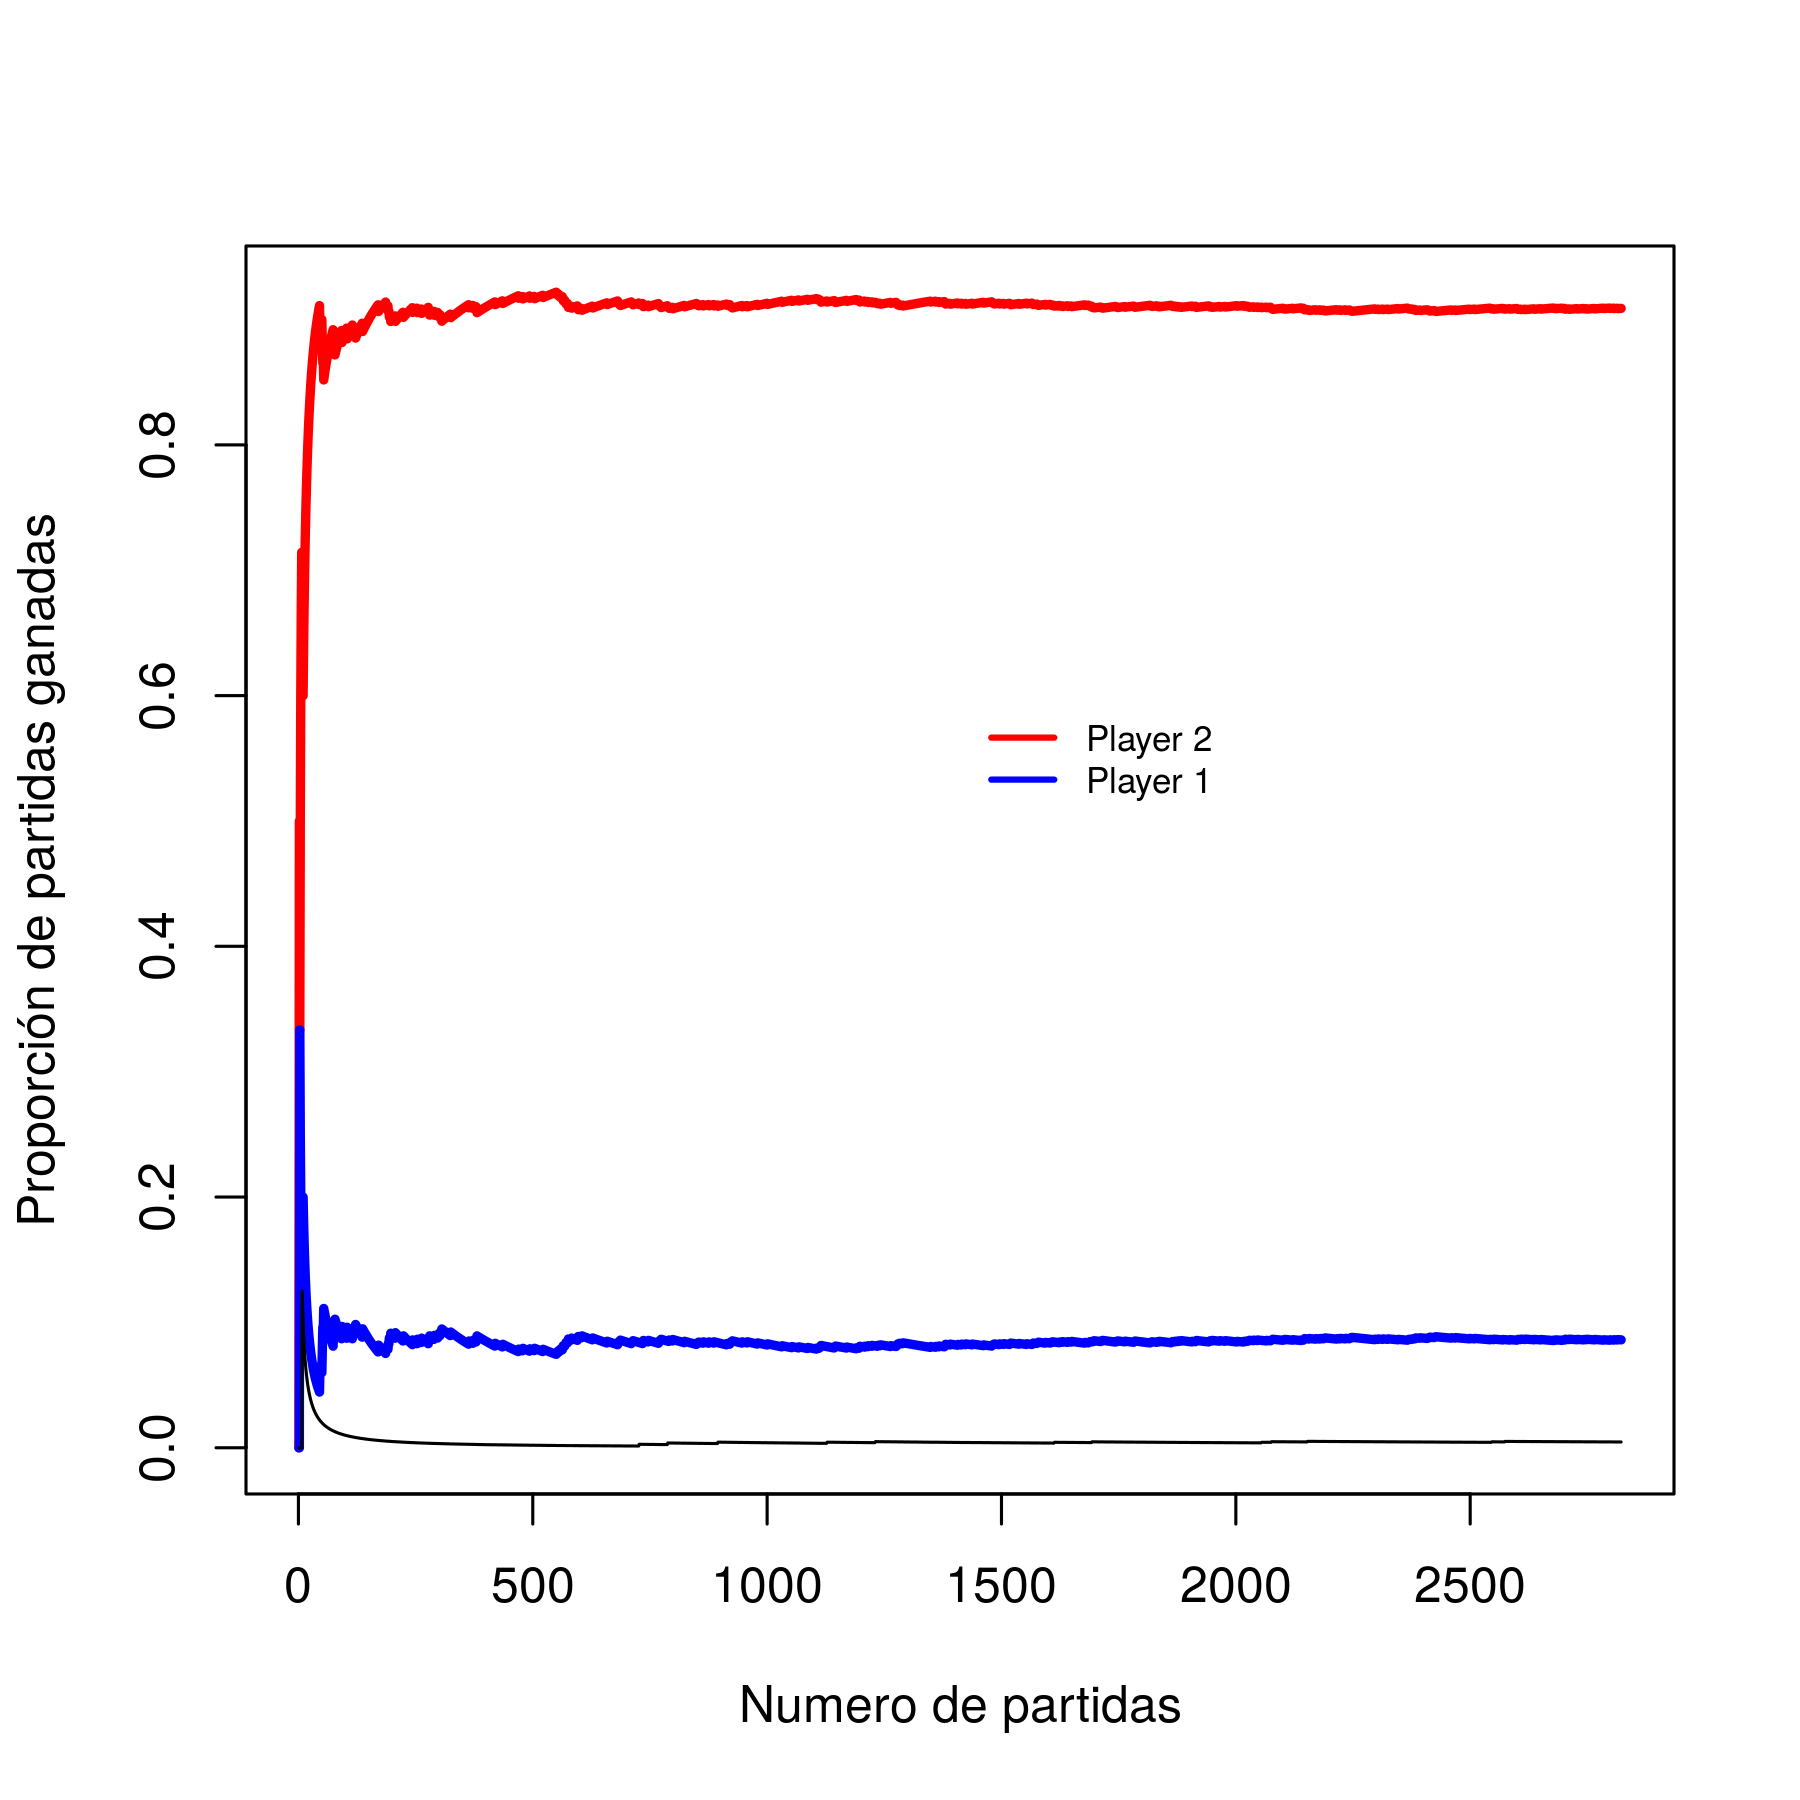
\includegraphics[width=\textwidth]{../Imagenes/SinVision_luchaNoLibre_QsinVison_reverse}
    \end{subfigure}
\end{figure}

\end{frame}


\begin{frame}{}


\begin{figure}[H]
    \centering
    \begin{subfigure}[b]{0.45\textwidth}
      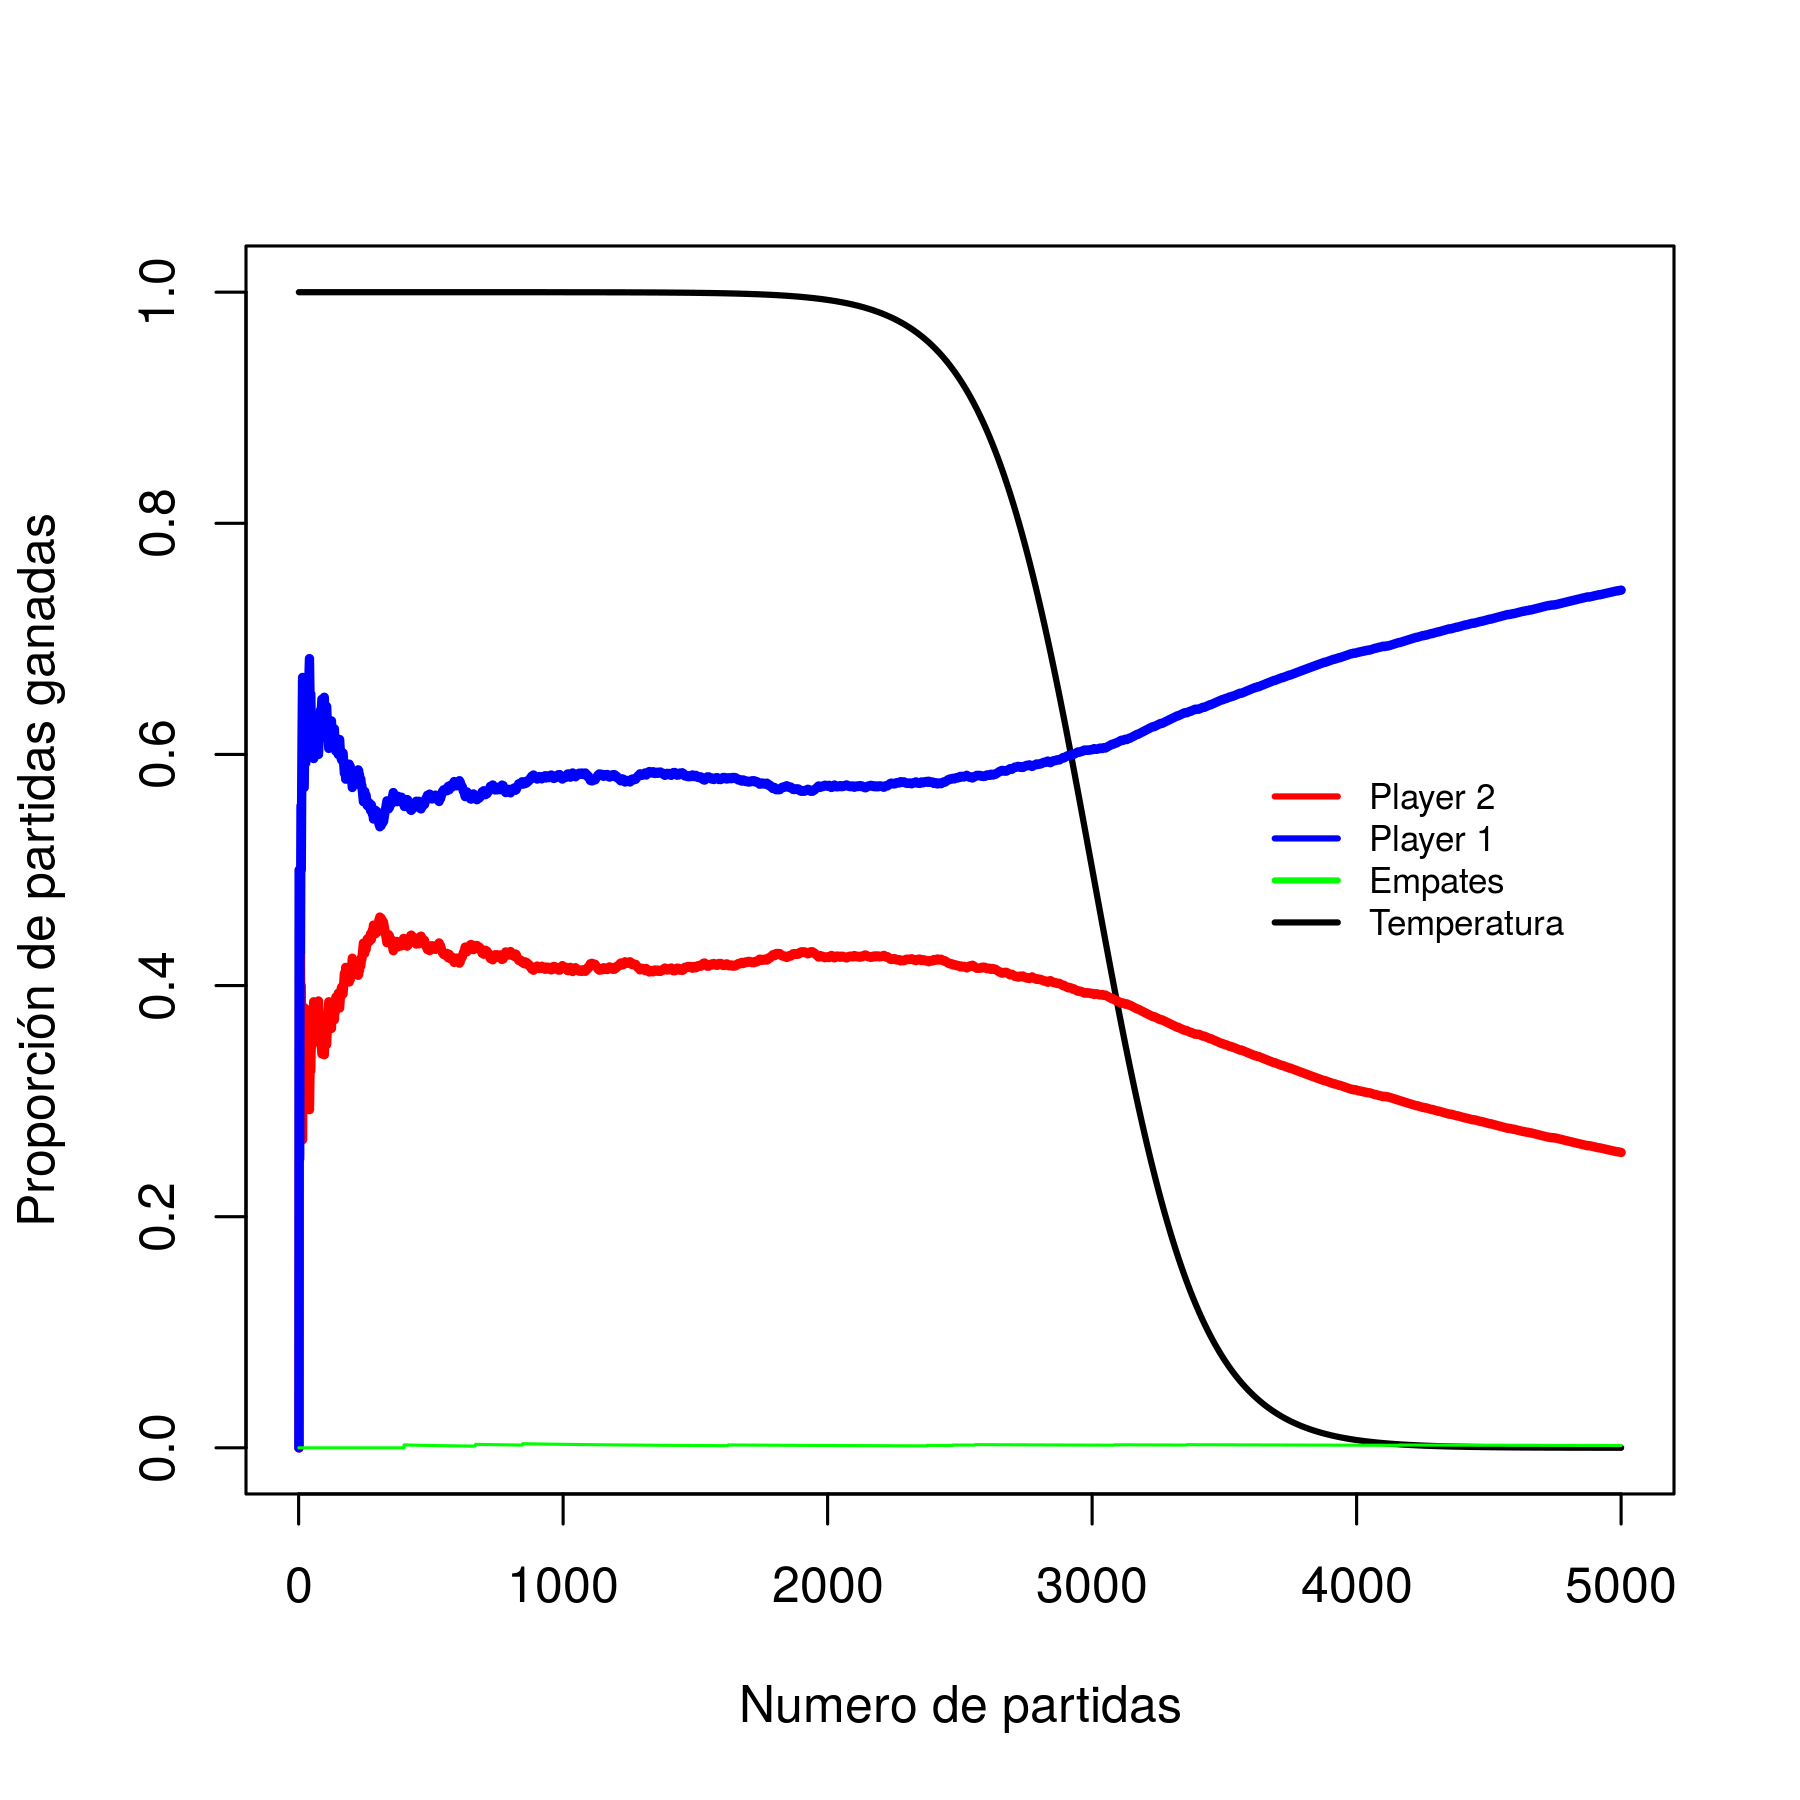
\includegraphics[width=\textwidth]{../Imagenes/SinVision_disipacion_QsinVison}
    \end{subfigure}
\end{figure}

\end{frame}


\begin{frame}{}


\begin{figure}[H]
    \centering
    \begin{subfigure}[b]{0.45\textwidth}
      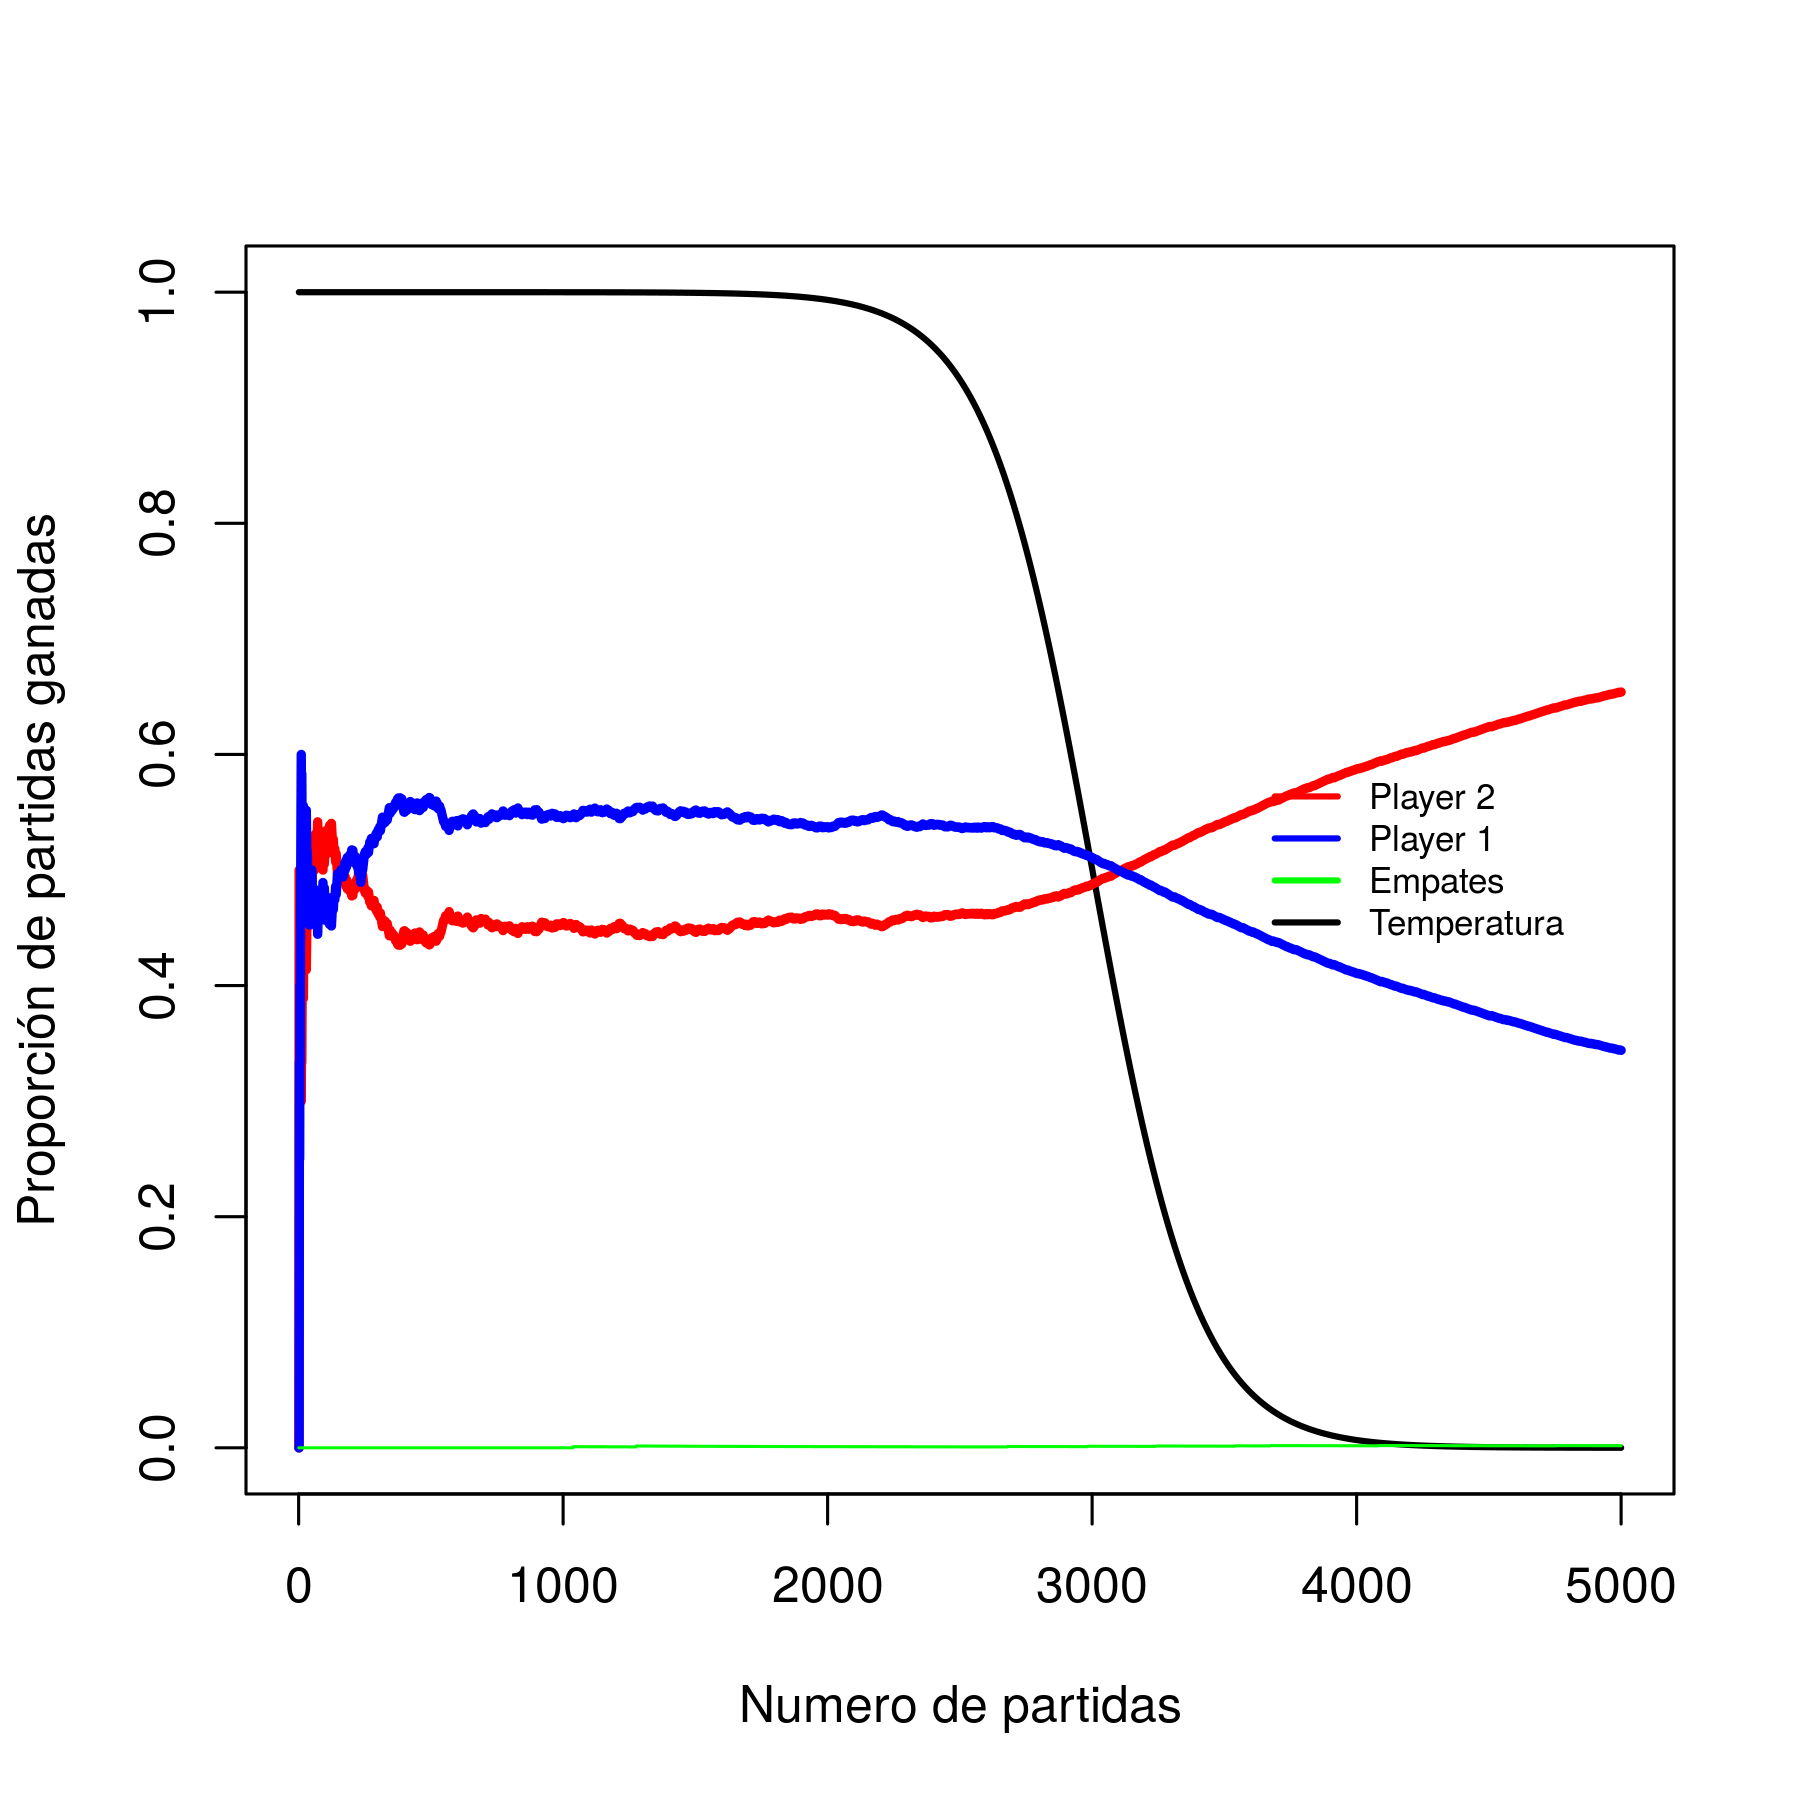
\includegraphics[width=\textwidth]{../Imagenes/SinVision_disipacion_QsinVison_reverse}
    \end{subfigure}
\end{figure}

\end{frame}


\begin{frame}{}


\begin{figure}[H]
    \centering
    \begin{subfigure}[b]{0.45\textwidth}
      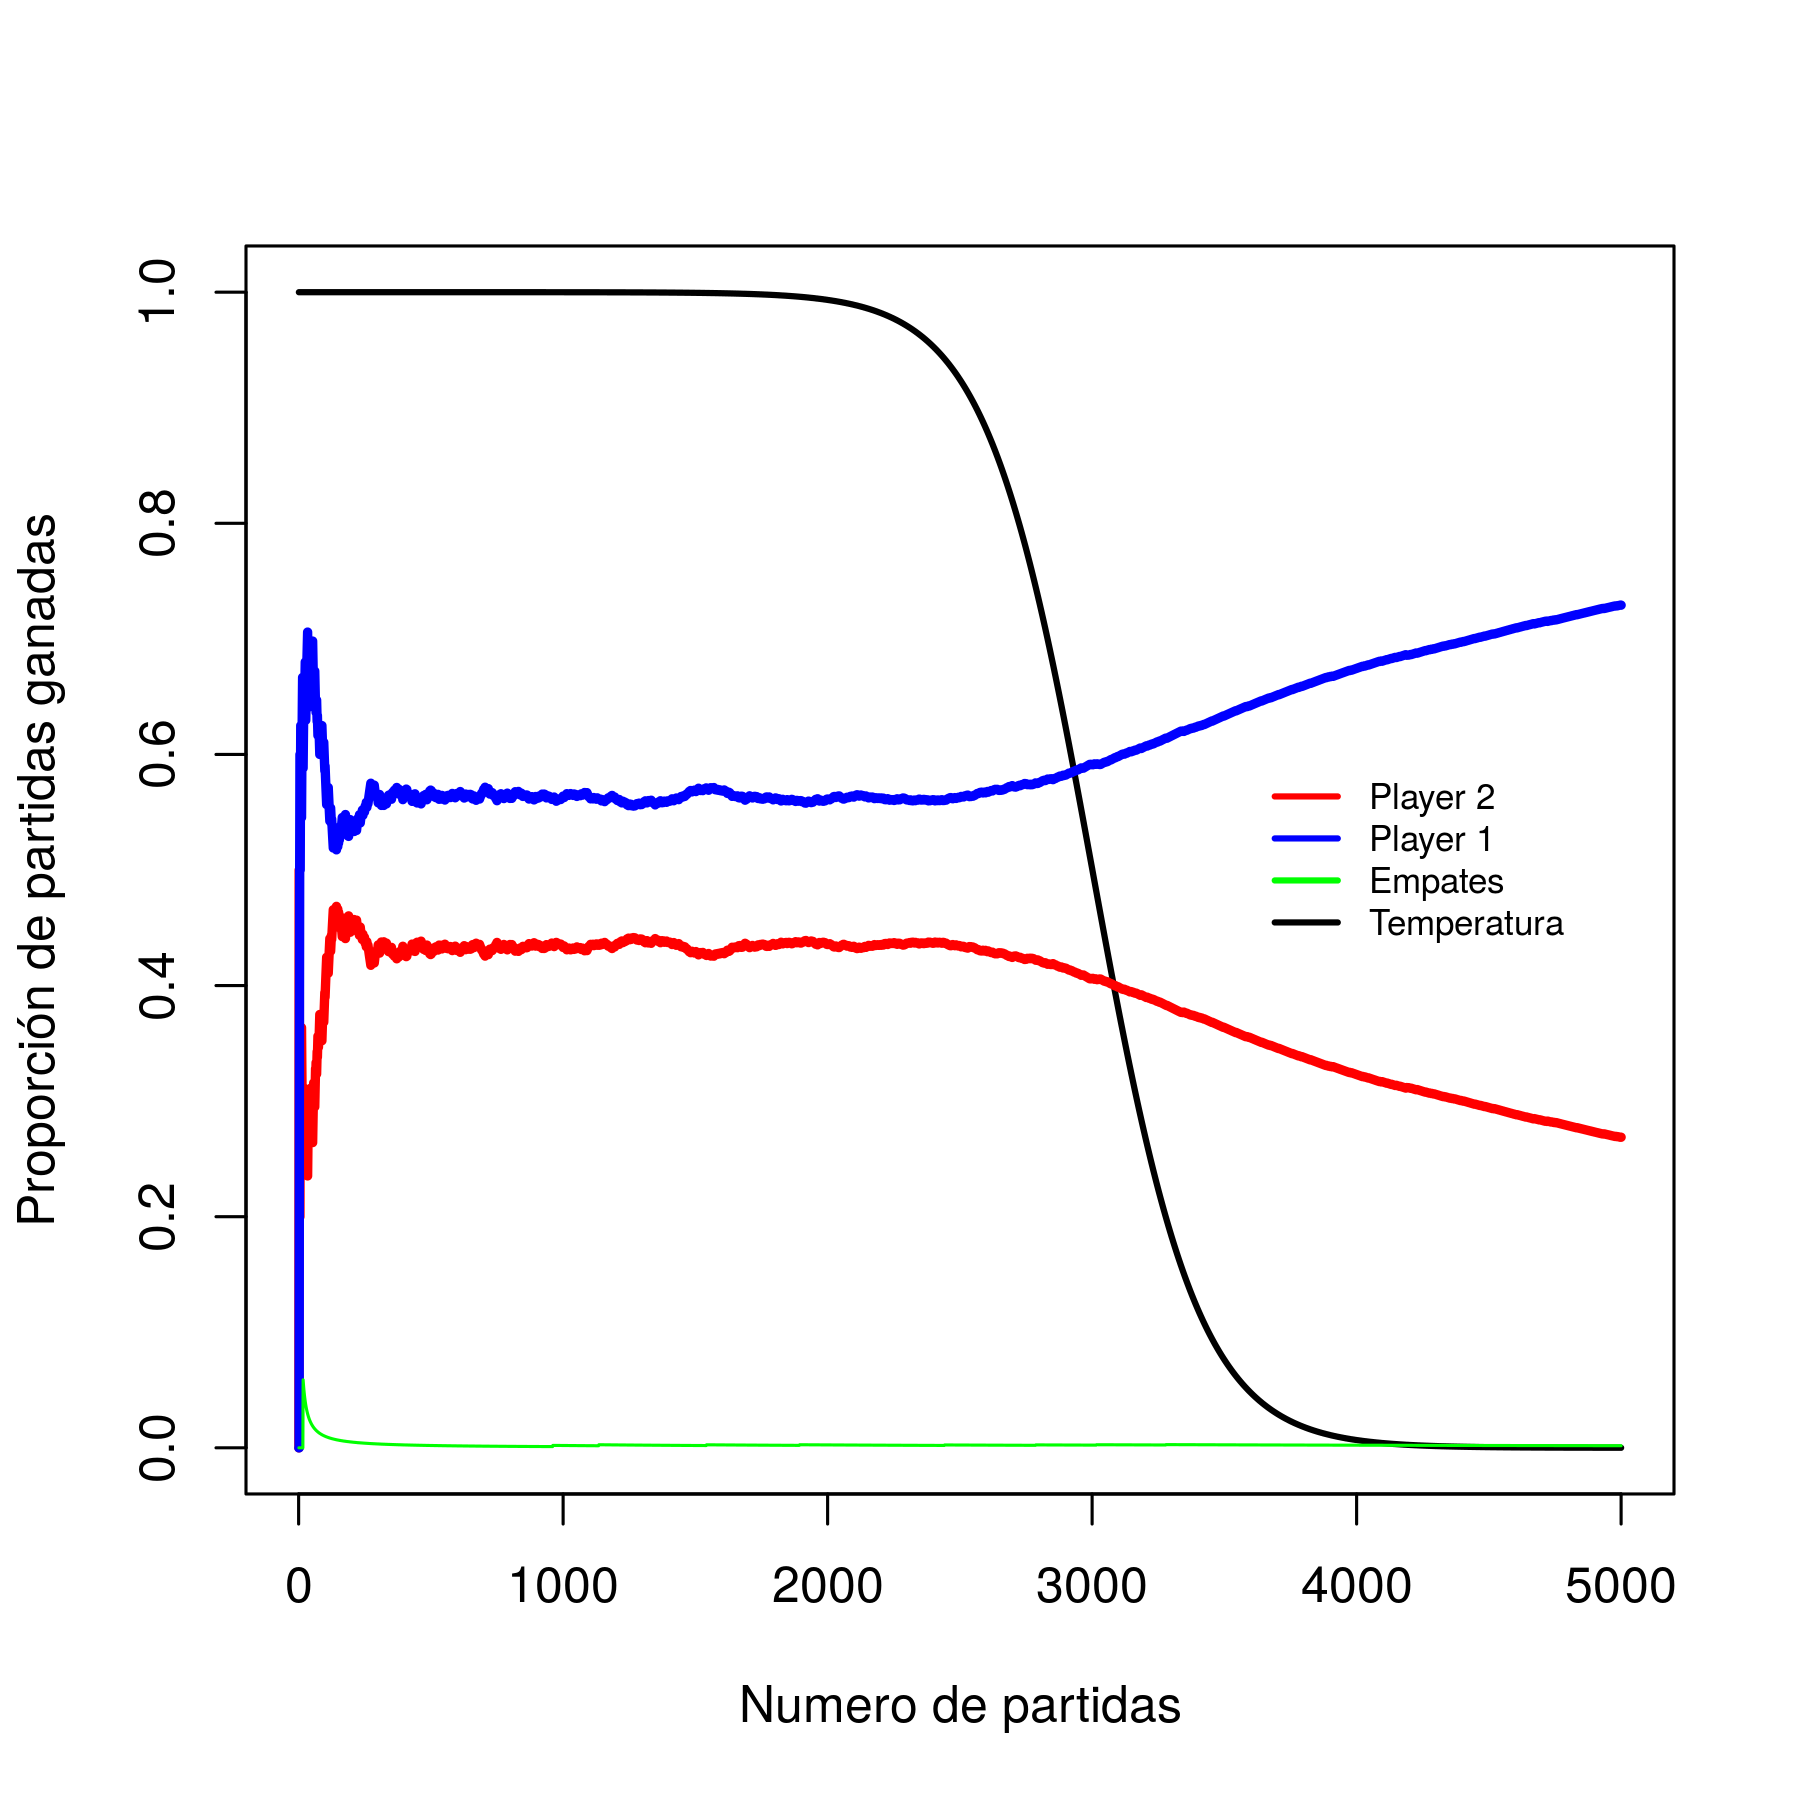
\includegraphics[width=\textwidth]{../Imagenes/SinVision_disipacion_QconVison}
    \end{subfigure}
\end{figure}

\end{frame}


\end{document}
